
\section{Results}
We summarize our findings over the created data streams. We ask whether lifelong pretraining and continual learning algorthms are effective base on our evaluation protocol proposed in Sec.~\ref{ssec:evaluation_protocols}. 
%\xiang{Let's post a few high-level analysis questions here to overview the section.}



% \xiang{Need an experiment setting or setup subsection to give some details: 1) eval metrics for different downstream tasks; 2) additional details about data streams and datasets; 3) implementation details, hps config, etc.}
\subsection{Experiment Settings}
We use the \texttt{RoBERTa-base} model~\cite{Liu2019RoBERTaAR}, initialized with RoBERTa-base weights throughout the experiments. We set the maximal sequence length to 128 and an effective training batch size of 2,048. On the research paper stream, models are trained for 8$k$ steps in the first domain and 4$k$ steps in the subsequent domains. On the Tweet stream, we train the models for 4$k$ steps in each domain. These correspond to less than a single pass of data in each domain. See Appendix~\ref{sec:hyps} for detailed setups. %\xiang{below details can move to appendix and leave a pointer here.}


% \subsection{Results on the Research Paper Stream}
\subsection{Domain Incremental Data Stream}
%\xiang{say a few sentences to re-cap the data stream setup and what aspects of model capability (i.e., measure of success) we're looking at here. Next, you can describe the exp setup/workflow as follows.}
As we introduced in Sec.~\ref{ssec:datasets}, in the domain incremental research paper stream, %the criterion is whether models can transfer knowledge to new domains while retaining knowledge in the domains visited earlier. 
we expect a model $f_t$ to perform well on all downstream tasks $S_{1..t}$ from domains $D_{1..t}$.
%\xiang{Still reads a bit vague to me; above can be further clarified using more notations.}
%\xiang{reference notations in Sec 2.1 to clarify more on the exp settings.}
In Table~\ref{tab:academics}, we report the performance of models on all downstream tasks $S_{1..T}$ fine-tuned from the final pretraining checkpoint, $f_T$. 
%For each downstream task related to a domain $D_t$, we fine-tune the language models at the time step $t$ and afterward, as indicated in the header ``evaluated after'' in Table~\ref{tab:academics}. 
We visualize more complete change of downstream task performance over different time steps of pretraining (\textit{i.e.,}, $f_1, f_2,f_3,f_4$) in Fig.~\ref{fig:academics_curve}. We also report the log perplexity of masked language modeling (MLM) in Table~\ref{tab:academics} as additional information. With these results, we address the research questions below.

%Table~\ref{tab:academics} summarizes the fine-tuning performance over the research paper data stream. 

% \xiang{\paragraph{\textit{Q1: Does sequential pretraining help retain knowledge across different domain corpora?}}
% (1) first talk about task-specific LM vs. roberta to show that domain corpus are useful for the corresponding downstream tasks;
% (2) see if Sequential Pretraining bring gains vs. task-specific LM --> if results are mix that mean that sequential pretraining (Sequential Pretraining) has space to be improved.
% }

%\xiang{Do we have anything special to say about MLM? I think the discrepancy between MLM and downstream performance are interesting to speak out?}

%\xiang{I don't see Fig~\ref{fig:academics_curve} being analyzed in details in any part now? I expect some interesting insights can be derived there.}

\paragraph{\textit{Does lifelong pretraining help retain knowledge across different domain corpora?}}
We first examine whether task-specific or lifelong pretraining improves performance over domain-specific downstream tasks. %\xiang{more clear if with notations}
Comparing Task-Specific LMs with RoBERTa-base in Table~\ref{tab:academics}, we notice consistent performance improvements, especially on Biomedical and Computer Science domains ($D_1, D_2$). %, where the F1-scores improve at least by 1.7\%. %Then most simple sequential pretraining apparoach, Sequential Pretraining, could also consistently improve over RoBERTa-base. 
% \paragraph{Performance Without CL Algorithms.} 
We also see Sequential Pretraining could consistently outperform RoBERTa-base. However, the comparison between Sequential Pretraining and Task Specific LMs are mixed: on $D_1, D_2, D_3$, Sequential Pretraining could outperform Task-Specific LMs only except MNER; while on the earliest biomedical domain ($D_1$), Sequential Pretraining achieves substantially lower performance. From Figure~\ref{fig:academics_curve}, we see the performance of Sequential Pretraining on Chemprot and RCT (from $D_1$) drops significantly from $t=1$ to $4$. %The results imply sequential pretraining still has space to be improved. \xiang{expand a bit more on the implication and how does it lead }
The results imply lifelong pretraining allows later domains to benefit from knowledge transfer from earlier domains, but the performance on earlier domains is limited because of forgetting.


% \paragraph{Comparison to Task-Specific Models.} 
%We find that Task-Specific LMs, which are trained independently over each domain-specific corpus, achieve comparable or sometimes better downstream performance than the best continually pretrained models. However, we argue that a clear advantage of continually pretrained models is that a single model can be applied to multiple domains.

\begin{table}[]
\centering
\scalebox{0.66}{
\begin{tabular}{@{}lccccc@{}}
\toprule
$|M|$, k       & Chemprot & RCT   & ACL-ARC & SciERC & MLM-$D_{1,2}$ \\ \midrule
$100k, 10$  & 82.73    & 79.98 & 72.50   & 81.64  & 1.737/1.857     \\
$100k, 100$ & 82.06    & 78.64 & 71.97   & 81.62  & 1.599/1.789     \\
$10M, 10$  & 82.87    & 79.98 & 71.80   & 81.63  & 1.438/1.732     \\ \bottomrule
\end{tabular}
}
\caption{\small Downstream task and MLM performance of $f_T$ under different memory sizes $|M|$ and the frequency of replay $k$ (replaying every $k$ steps of training) in ER.}
\label{tab:er_tune}
\vspace{-0.2cm}
\end{table}


\paragraph{\textit{Does continual learning algorithms help retain knowledge in sequential pretraining?}}
Next, we compare different kinds of CL algorithms and investigate the effect of CL algorithms in alleviating forgetting and improving knowledge transfer. %.\xiang{elaborate more on the goal and overview here. Effect on what? What effects?}
% \paragraph{Effect of Adapter Approaches.} 
%\xiang{1) Where do readers look for these observations? 
%2) Note that Table 1 is special as it is for LM from the last domain/step -- therefore it makes sense that 
%3) I found the last two sentences here most interesting; other detailed observations can be compress to brief summary to save space.}
Table~\ref{tab:academics} shows that Online-EWC slightly improves MLM perplexity compared to  Sequential PT, but brings no improvement to the fine-tuning performance. We hypothesize that regularization directly in the parameter space as in Online-EWC is not effective when the parameter space is very high dimensional.
%We first compare the performance of model architecture based approaches with Sequential Pretraining.
Adapter improves downstream task F1 scores on the bio-medical domain ($D_1$) by 1.2\% and 0.8\%, 
but does not outperform Sequential Pretraining in other domains (similarly for Simple Layer Expansion approach), %We note that despite the immunity to forgetting of model expansion approaches, these methods struggle to outperform simple Sequential Pretraining, %. The reason is likely to be the reduced modeling capacity for new domains
likely because a great portion of the model is kept frozen. % in these approaches. 


\begin{figure*}[!t]
    \centering
    % \scalebox{0.9}{
    \subfloat[\scriptsize{Chemprot}]{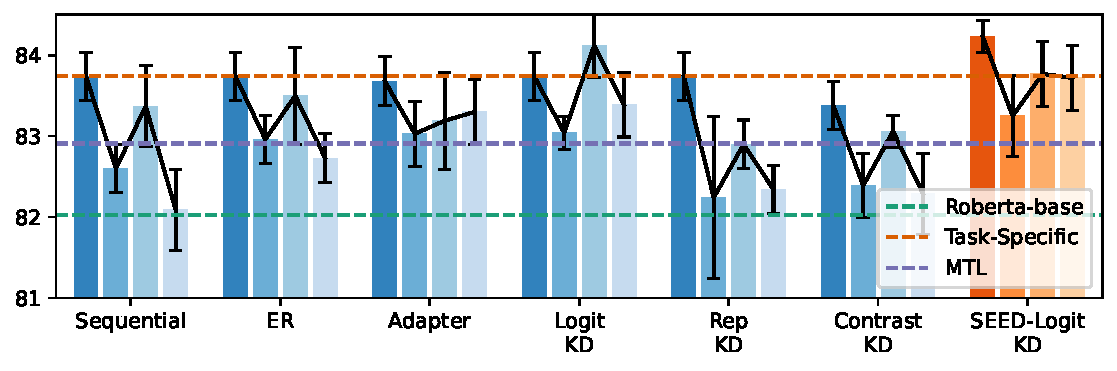
\includegraphics[width=0.48\linewidth]{acl2022/figs/academics_plots/Chemprot.pdf}}
    \subfloat[\scriptsize{RCT-Sample}]{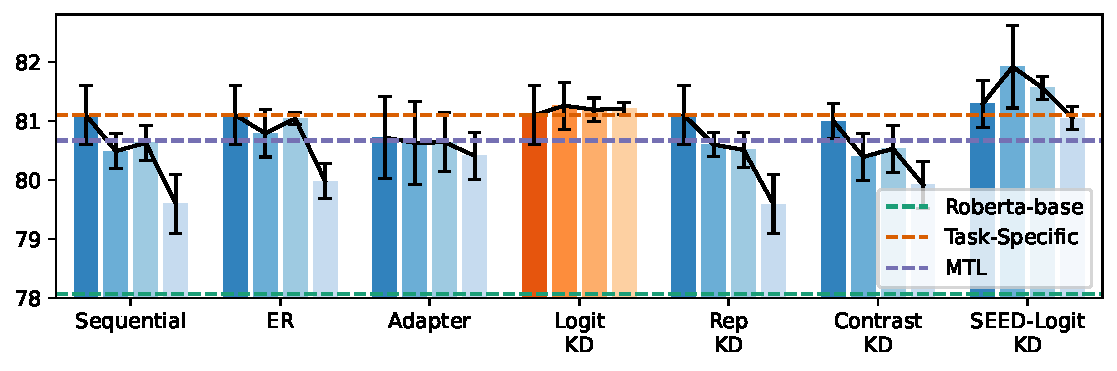
\includegraphics[width=0.48\linewidth]{acl2022/figs/academics_plots/RCT-Sample.pdf}}


    \subfloat[\scriptsize{ACL-ARC}]{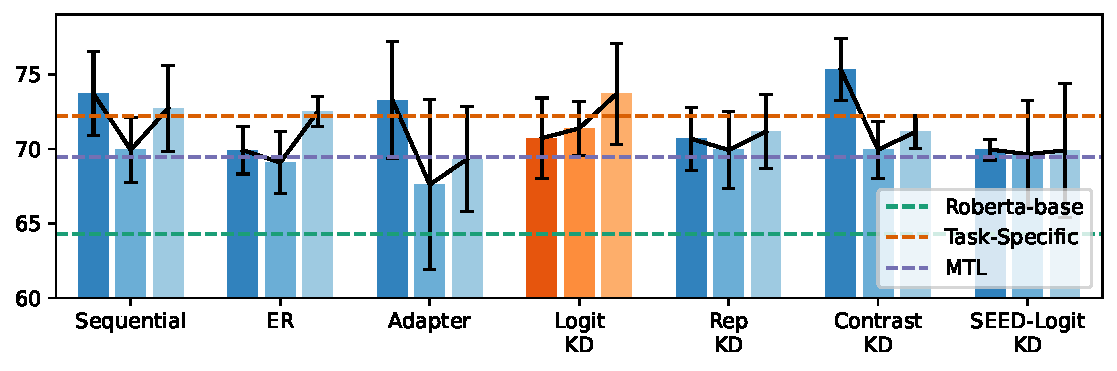
\includegraphics[width=0.48\linewidth]{acl2022/figs/academics_plots/ACL-ARC.pdf}}
    \subfloat[\scriptsize{SciERC}]{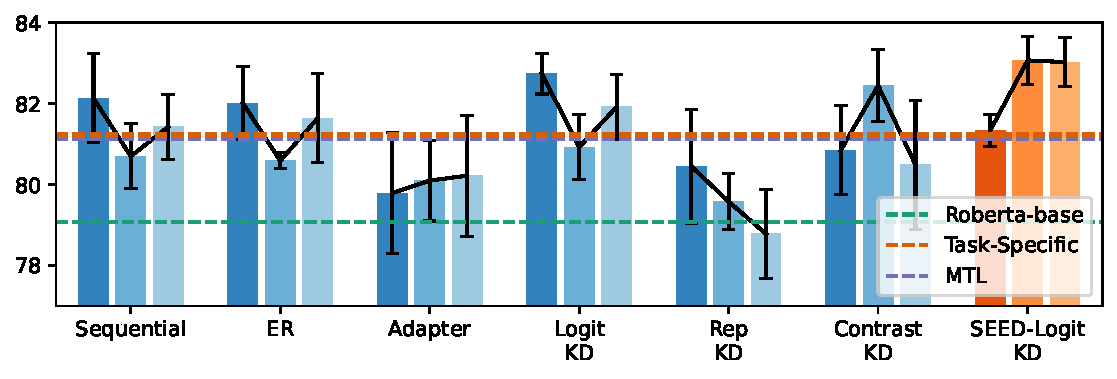
\includegraphics[width=0.48\linewidth]{acl2022/figs/academics_plots/SciERC.pdf}}
    % }
    \caption{\small \textbf{Performance evolution of downstream models.} Models are fine-tuned from checkpoints of lifelong pretrained LMs at different time steps $t$. For Chemprot and RCT-Sample from $D_1$, we use $t \in \{1,2,3,4\}$; while for ACL-ARC and SciERC from $D_2$, $t \in \{2,3,4\}$. Methods achieving the best performance at the end of training ($t=4$) is highlighted.}
    \label{fig:academics_curve}
    \vspace{-0.3cm}
\end{figure*}


\begin{figure}[]
    \centering
    % \scalebox{0.9}{
    %\subfloat[\scriptsize{Chemprot}]{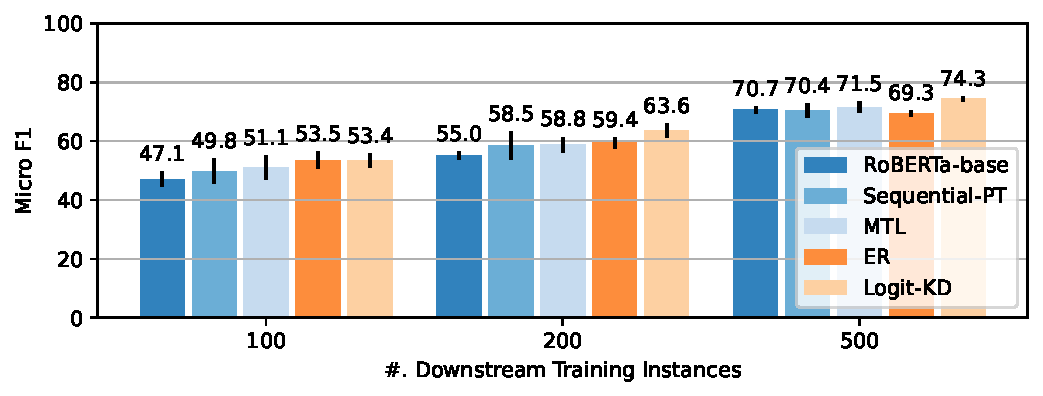
\includegraphics[width=0.94\linewidth]{acl2022/figs/academics_kshots/kshot_chemprot.pdf}}
    %\vspace{-0.3cm}
    %\subfloat[\scriptsize{RCT-Sample}]{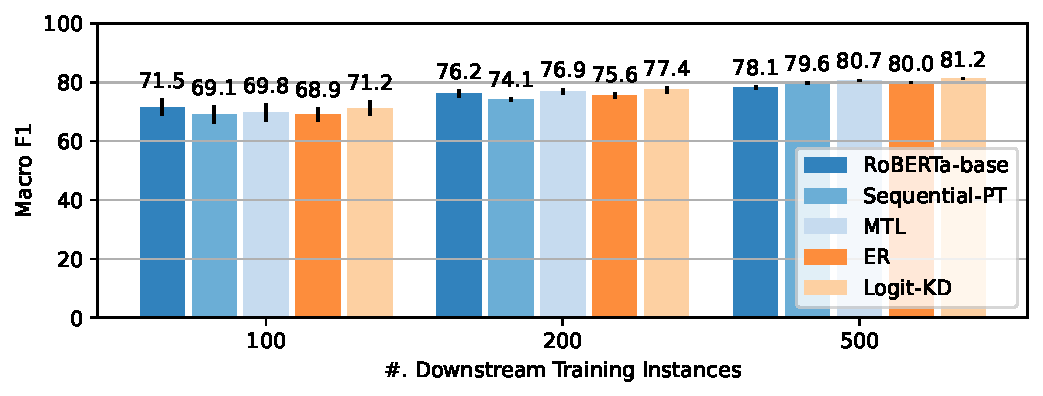
\includegraphics[width=0.94\linewidth]{acl2022/figs/academics_kshots/kshot_rct-sample.pdf}}
    %\vspace{-0.3cm}
    %\subfloat[\scriptsize{ACL-ARC}]{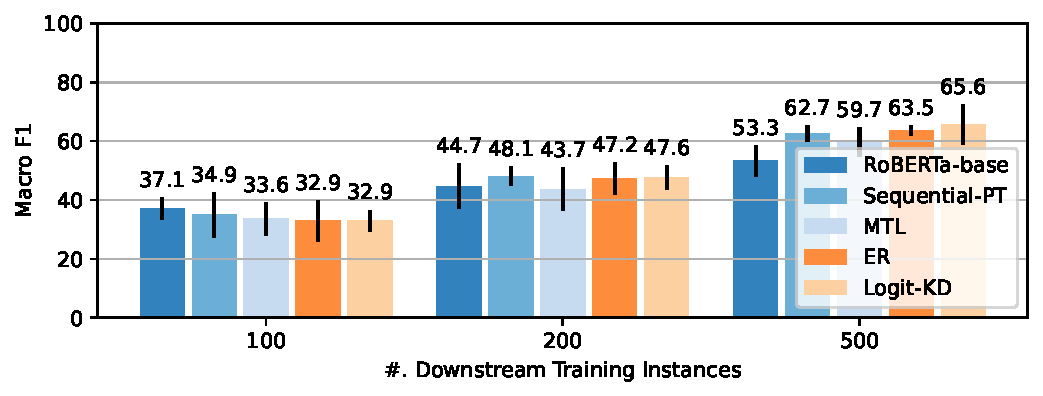
\includegraphics[width=0.94\linewidth]{acl2022/figs/academics_kshots/kshot_citation_intent.pdf}}
    % \vspace{-0.3cm}
    
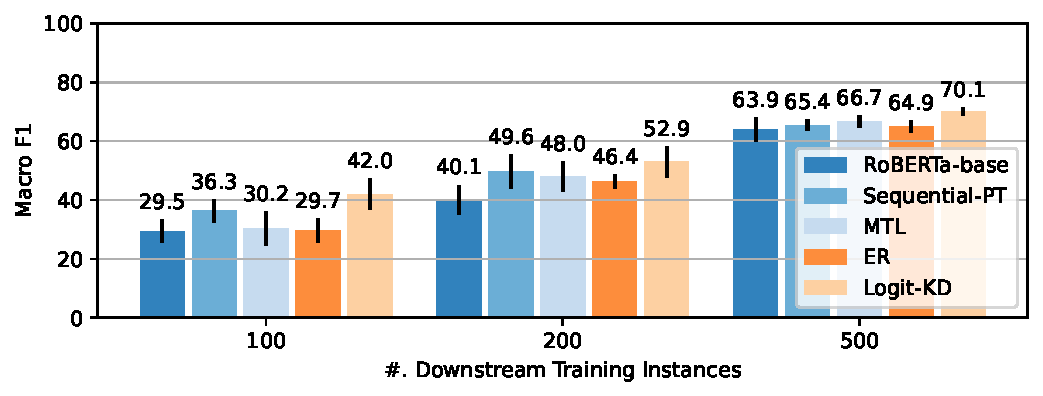
\includegraphics[width=0.98\linewidth]{acl2022/figs/academics_kshots/kshot_sciie.pdf}
    % }
    \caption{\small \textbf{Performance of downstream models with various number of training examples}, exemplified with SciERC. The models are fine-tuned from the final pretrained model ($f_4$).}
    \label{fig:academics_kshot_subset}
\end{figure}




% \paragraph{Effect of Experience Replay.} 
%\xiang{smooth out transition and recap the pros and cons of memory based methods.}
In contrast, the memory-replay based approach (ER) allows training the full parameters of the model and has been shown to be highly effective in continual learning of classification tasks~\cite{Wang2019SentenceEA, chaudhry2019tiny}. However, we surprisingly find that ER could hardly improve over Sequential Pretraining except $D_1$. % by 0.6\% and 0.4\%.
A similar pattern can be found in the MLM perplexity. 
We hypothesize that the positive effect of example replay has diminished because of the overfitting to the memory examples. Table~\ref{tab:er_tune} summarizes the effect of tuning hyperpameters in ER. When we reduce the frequency of replay (from every 10 steps to 100 steps), the MLM performance improves, which implies reduced overfitting; however, the performance of downstream task performance does not improve. When we increase the size of the memory $|M|$ from $100k$ to $10M$, the MLM perplexity also improves; still, there are still no improvements in downstream tasks. It may imply ER itself is not an effective approach for continual pretraining. %We leave more analysis into ER as future works. %We further examine the performance of ER when we experiment with a larger replay memory but notice marginal improvements, detailed in Appendix.

%\xiang{smooth out transition and recap the pros and cons of KD methods.}


Unlike ER, distillation approaches utilize richer information such as output logits or representation similarity to preserve past knowledge. We find either Logit KD or SEED-Logit KD to be most effective depending on the task, while Rep-KD and Contrastive-KD are less effective. The best performing distillation approach improves F1 over Sequential Pretraining on downstream tasks from $D_1$, $D_2$ at least by 1.0\%. However, performance on $D_3, D_4$, which come later in the data stream, does not improve over Sequential Pretraining, possibly because the distillation loss term %which tries to retain models' past knowledge 
makes the model rigid in obtaining new knowledge.

%because retaining past knowledge is a burden for obtaining new knowledge while the model has not yet suffered significantly from forgetting at the end of pretraining. 
%Still, the performance on MNER, Synthesis and Hyponym improve over the RoBERTa-base model. 
%Other distillation algorithms, such as Rep-Distill and Contrast-Distill, were not as effective as Logit-Distillation or SEED-Distillation. %However, from the performance evolution of downstream models at different pretraining checkpoint illustrated in Figure~\ref{fig:academics_curve}, we see SEED-Logit Distill could occasionally outperform Logit-Distill (\textit{e.g.,} on RCT-Sample), but in general does not outperform Logit-Distill. It implies their can be positive effect of preserving similarity structure of representations in additional to model outputs, but the effect is highly dependent on the task. 

% \paragraph{Effect of Distillation Approaches.}
%From the performance of Logit Distillation, Representation Distillation, and Contrastive Distillation, we find that only Logit Distillation could clearly reduce masked language modeling perplexity over the baselines. Representation and Contrastive Distillation do not reduce masked language modeling perplexity, which is understandable, because these two algorithms directly operate over the sentence representations, leaving the masked language model prediction head unregularized. However, we further find that only Logit distillation could consistently improve downstream task performance over Sequential Pretraining on downstream tasks in earlier domains when evaluated at the end of pretraining. The results indicate that Logit Distillation is a highly effective algorithm, and also implies that input logits are useful dark knowledge for knowledge preservation. We note the current results do not necessarily imply that the stability of representations and representational similarity is irrelevant to alleviating forgetting. In future works, we may further improve the loss term of distillation applied in Representation and Contrastive distillation.

%\xiang{Addition Analysis/discussion on ER: show the performance trend of ER wrt the size of memory, and convince people that to get little performance improvement it requires a lot larger memory, and thus less data efficient as compared to the KD methods.}

\begin{table*}[]
\centering
\scalebox{0.70}{
\begin{tabular}{@{}lccccc@{}}
\toprule
Method                                     & \#. of Forward & \#. of Backward & \#. Total   & \#. Total ($k$=10) & \ Wall Time$_{4k}$ \\ \midrule
\textit{Main results}                      &                          &                            &            &      &     \\
Sequential PT                              & $b$                      & $b$                        & $2b$       & $2b$   &  $4.0\times 10^4$ sec.  \\
ER                                         & $(1+1/k)b$               & $(1+1/k)b$                 & $(2+2/k)b$ & $2.2b$ & $4.2\times 10^4$ sec.  \\
Logit-Distill                              & $(2+2/k)b$               & $(1+1/k)b$                 & $(3+3/k)b$ & $3.3b$ &  $6.9\times 10^4$ sec.  \\
SEED-Logit-Distill                         & $(3+3/k)b$               & $(2+2/k)b$                 & $(5+5/k)b$ & $5.5b$  & $9.7\times 10^4$ sec.\\
\midrule
\textit{Additional Controlled Experiments} &                          &                            &            &        &  \\
Sequential PT$_{b^\prime=1.2b}$                     & $1.2b$                   & $1.2b$                     & $2.4b$     & $2.4b$  &  $4.4 \times 10^4$ sec. \\
%Sequential PT$_{b^\prime=1.65b}$                     & $1.65b$                   & $1.65b$                     & $3.3b$     & $3.3b$  &   \\
ER$_{k=5}$   & $1.2b$                   & $1.2b$                     & $2.4b$     & $2.4b$  &  $4.4 \times 10^4$ sec.  \\
Sparse Logit-KD                            & $1.3b$                  & $1.1b$                    & $2.4b$     & $2.4b$  & $4.4 \times 10^4$ sec.  \\
Sparse SEED-Logit-KD$_{\backslash contrast}$         & $1.3b$                  & $1.1b$                    & $2.4b$     & $2.4b$  &  $4.8 \times 10^4$ sec. \\ \bottomrule
\end{tabular}
}
\caption{Number of forward and backward passes over PTLMs and wall clock time of different approaches. The number of forward and backwards passes are computed over visits of $b$ batches from the training data stream, where $k$ is the frequency of replay. The wall clock time is calculated over 4$k$ steps of training (which is the number of training steps of a single domain in the Research Paper stream) excluding the first domain, as no replay or distillation happens while learning the first domain. In the additional controlled experiments (described in~Appendix.~\ref{apdx:controlled_computation_costs}), we control the total number of forward and backward passes of different approaches. %This also yields approximately the same wall clock time for approaches.
}
\label{tab:forward_backward_count}
\end{table*}






\paragraph{\textit{What is the gap between lifelong pretraining and multi-task learning across all the domains?}
%This needs comparison with multi-task pretraining baseline --- If we can do CL pretraining well, can CL be comparable to multi-corpus pretraining. If so, we can do CL which is much cheaper than MTL.
}
%\xiang{first say a bit on the motivation and hypothesis behind this analysis.}
Multi-Task Learning refers to the offline training paradigm, which retrain PTLMs over all corpora ($D_{1..t}$) each time a new corpus $D_t$ becomes available. 
%The practice is computationally expensive if new corpora keep emerging. 
We examine whether lifelong pretraining is comparable to multi-task pretraining in terms of performance. From Table~\ref{tab:academics} and Figure~\ref{fig:academics_curve}, we see Sequential Pretraining in general underperforms MTL except for the final domain. However, certain CL approaches, such as Logit-Distillation, could improve over MTL on all downstream tasks from the first and the second domain. We speculate the reason is that continual learning naturally provides a curriculum~\cite{Xu2020CurriculumLF, Shi2015RecurrentNN} to models where each individual task is easier to learn. 
%, in contrast to MTL, where data is mixed from multiple domains. 
The results have a positive implication that lifelong pretraining is not only more computationally efficient and requires less storage of past data, but may also improve the performance of pretraining.



\paragraph{\textit{Does lifelong pretraining make models more data efficient?}}
In Table~\ref{fig:academics_kshot_subset}, we further examine the performance of final pretrained models under different amounts of training examples. We include full results in Appendix~\ref{apdx:low_resource}. We find in general, performance improvements are more significant in the low-resource setup. %\xiang{revise and expand a bit more on the msgs.}
%We hypothesize it is because the accumulated knowledge over continual pretraining creates a better model initialization to help learn downstream tasks in a more data-efficient manner.



\paragraph{\textit{Computational Costs.}} We quantify computational costs of different CL algorithms with the number of forward and backward passes in Table~\ref{tab:forward_backward_count} and present additional experiments with controlled computational costs in Appendix~\ref{apdx:controlled_computation_costs}. We find additional computational cost is necessary for performance improvement of distillation-based CL. However, it is not possible to trade performance simply by investing more computation budget with arbitrary CL algorithms. We leave detailed discussions in Appendix~\ref{apdx:controlled_computation_costs}.

%Exp 2 Setup (fine-tuning data efficiency): take checkpoints from (original LM, task-specific LM, CL-LM); do fine-tuning and track the performance wrt fine-tuning steps.
%}







\subsection{Temporal Data Stream}
\label{ssec:temporal_data_stream}

We conduct analysis on pretraining PTLM on chronologically-ordered tweet corpora, to understand whether lifelong pretraining helps adaptation to the latest data and improves temporal generalization ability. %In this setup, the pretrained corpora $D_{1..4}$ are tweet data in different years%and the pretrained LMs are fine-tuned on Hashtag and Emoji prediction data from each year of $D_{1..4}$.
% We then move our focus to the next set of research questions regarding whether lifelong pretraining improves model's adaptation to latest data and temporal generalization when the data stream is chronologically ordered.
%\xiang{add 1-2 sentences on overview of the exp setup?}
%We study a series of research questions using the tweet stream. 
The results are summarized in Table~\ref{tab:twitter}.
% We summarize our findings below.

%\xiang{\paragraph{\textit{Q1: Will LM be outdated?}}
%updated LM vs. original LM
%}
\paragraph{\textit{Will LMs be outdated?}} %We first examine whether the LM pretrained specifically on the tweets of 2014 (the row of Task-Specific (2014) in Table~\ref{tab:twitter}) becomes less effective when applied to downstream datasets from subsequent years. 
We compare the performance of Task-Specific (2014) to the Task-Specific models pretrained on the year of downstream datasets (noted as Task-Specific (Latest)) and notice consistent improvements in downstream tasks in 2018 and 2020  (first two columns in Table~\ref{tab:twitter}). Sequential Pretraining could also outperform the Task-Specific (2014) model. It verifies that language models may get outdated over time, but the issue can be addressed by task-specific or lifelong pretraining over the latest corpora.

% As we mentioned in Sec.~\ref{ssec:evaluation_protocols}, over chronologically ordered data streams, the performance over the latest data is of higher importance. Therefore, in Table~\ref{tab:twitter}, we focus on the hashtag prediction performance in the year 2020. Unfortunately, we find continually pretrained models do not improve over task-specific models, which are only pretrained over the latest year. It may imply knowledge from earlier years is redundant for the hashtag prediction task given the latest data. 

\begin{table}[]
\centering
\scalebox{0.607}{
% Please add the following required packages to your document preamble:
% \usepackage{booktabs}
\begin{tabular}{@{}lcccc@{}}
\toprule
Years                  & 2018 $(D_3)$              & 2020 $(D_4)$              & \begin{tabular}[c]{@{}c@{}}2014 $(D_1)$ \\ $\to$ 2020 $(D_4)$\end{tabular} & \begin{tabular}[c]{@{}c@{}}2016 $(D_2)$\\ $\to$ 2020 $(D_4)$\end{tabular} \\ \midrule
\multicolumn{5}{c}{Hashtag Prediction}                                                                   \\ \midrule
RoBERTa-base           & 48.08$_{\pm 1.0}$ & 56.42$_{\pm 0.2}$  & 39.31$_{\pm 2.7}$ & 42.23$_{\pm 2.7}$ \\
Sequential PT          & 56.79$_{\pm 0.5}$ & 59.85$_{\pm 0.4}$  & 44.00$_{\pm 1.1}$ & 49.87$_{\pm 1.8}$ \\
ER                     & 56.93$_{\pm 0.1}$ & 59.56$_{\pm 1.7}$  & 43.31$_{\pm 0.2}$ & 50.72$_{\pm 0.6}$ \\
%Adapter                & 54.34$_{\pm1.7}$  & 59.01$_{\pm 1.0 }$ & 42.61$_{\pm 0.5}$ & 48.00$_{\pm 1.6}$ \\
Logit-KD               & \textbf{58.21$_{\pm 0.5}$} & 60.52$_{\pm 0.2}$  & 44.26$_{\pm 0.9}$ & 50.92$_{\pm 0.8}$ \\
%Rep-KD                 & 55.79$_{\pm 1.4}$ & 59.80$_{\pm 0.2}$  & 42.48$_{\pm 0.2}$ & 50.38$_{\pm 1.5}$ \\
Contrast-KD            & 57.94$_{\pm 0.4}$ & 59.54$_{\pm 0.3}$  & 45.22$_{\pm 0.1}$ & \textbf{52.14$_{\pm 1.1}$} \\
SEED-KD                & 56.87$_{\pm 0.2}$ & 59.71$_{\pm 0.2}$  & 43.39$_{\pm 0.4}$ & 49.62$_{\pm 1.0}$ \\
SEED-Logit-KD          & 57.75$_{\pm 0.4}$ & \textbf{60.74$_{\pm 0.6}$}  & \textbf{45.35$_{\pm 0.6}$} & 51.56$_{\pm 0.7}$ \\  \midrule
Task-Specific (2014)   & 56.16$_{\pm 0.6}$ & 59.59$_{\pm 0.3}$  & 44.34$_{\pm 0.6}$ & 49.26$_{\pm 0.7}$ \\
Task-Specific (Latest) & 56.61$_{\pm 0.4}$ & 59.87$_{\pm 0.6}$  & 43.44$_{\pm 0.5}$ & 49.41$_{\pm 1.1}$ \\
MTL                    & 57.89$_{\pm 0.4}$ & 59.95$_{\pm 0.3}$  & 44.04$_{\pm 0.3}$ & 50.37$_{\pm 0.3}$ \\
\midrule
\multicolumn{5}{c}{Emoji Prediction}                                                                     \\ \midrule
RoBERTa-base           & 25.71$_{\pm 0.1}$ & 24.42$_{\pm 0.2}$  & 12.02$_{\pm 0.4}$ & 13.24$_{\pm 0.2}$ \\
Sequential PT          & 29.30$_{\pm 0.1}$ & 27.69$_{\pm 0.1}$  & 14.20$_{\pm 0.2}$ & 16.08$_{\pm 1.4}$ \\
ER                     & 29.50$_{\pm 0.1}$ & 27.75$_{\pm 0.1}$  & 14.36$_{\pm 0.4}$ & 16.82$_{\pm 0.3}$ \\
%Adapter                & 28.72$_{\pm 0.0}$ & 26.80$_{\pm 0.3}$  & 13.53$_{\pm 0.2}$ & 15.68$_{\pm 0.3}$ \\
Logit-KD               & 29.77$_{\pm 0.1}$ & 27.80$_{\pm 0.1}$  & 14.20$_{\pm 0.3}$ & 16.28$_{\pm 1.1}$ \\
%Rep-KD                 & 29.45$_{\pm 0.1}$ & 27.27$_{\pm 0.2}$  & 13.89$_{\pm 0.1}$ & 16.03$_{\pm 0.3}$ \\
Contrast-KD            & 29.48$_{\pm 0.2}$ & 27.72$_{\pm 0.3}$  & \textbf{14.42$_{\pm 0.3}$} & \textbf{17.52$_{\pm 0.1}$} \\
SEED-KD                & \textbf{30.12$_{\pm 0.1}$} & 27.66$_{\pm 0.1}$  & 14.36$_{\pm 0.1}$ & 16.97$_{\pm 0.4}$ \\
SEED-Logit-KD          & 29.98$_{\pm 0.1}$ & \textbf{27.84$_{\pm 0.2}$}  & 14.36$_{\pm 0.1}$ & 16.97$_{\pm 0.3}$ \\ \midrule
Task-Specific (2014)   & 28.94$_{\pm 0.0}$ & 26.98$_{\pm 0.2}$  & 13.39$_{\pm 0.2}$ & 15.14$_{\pm 0.2}$ \\
Task-Specific (Latest) & 29.06$_{\pm 0.2}$ & 27.19$_{\pm 0.1}$  & 13.00$_{\pm 0.2}$ & 14.48$_{\pm 0.3}$ \\
MTL                    & 29.52$_{\pm 0.2}$ & 27.47$_{\pm 0.0}$  & 14.07$_{\pm 0.2}$ & 16.64$_{\pm0.2}$   \\  \bottomrule
\end{tabular}
}
\caption{\small \textbf{Results on temporal data stream.} We show fine-tuning performance over years 2018 and 2020 ($D_3$, $D_4$) and the Temporal generalization from 2014 or 2016 to 2020 data ($D_1\to D_4$, $D_2 \to D_4$) on Twitter Hashtag and Emoji prediction datasets. Models are fine-tuned from the final pre-trained model $f_T$. We include full results on other years ($D_1$, $D_2$, $D_3 \to D_4$) in Appendix~\ref{apdx:full_tweet_results}.
%\texttt{Year 1}$\to$\texttt{Year 2} indicates the hashtag prediction model is fine-tuned on data in year \texttt{Year 1}, and evaluated on test data in \texttt{Year 2}.
}
\label{tab:twitter}
\end{table}



\paragraph{\textit{Does lifelong pretraining help improve the downstream model’s performance on latest data?}}
%\xiang{1) Where (what part of results) to look for the observations? (do we look for year 2020, or all years, or sth else?)
%2) What is the main takeaway distilled in an accessible sentence? Can we have that up front?
%}
We show that downstream model's performance over later data ($D_3, D_4$) can be improved over Task-Specific models when continual learning algorithms are applied. From the first two columns of Table~\ref{tab:twitter}, %we see no consistent improvement of simple Sequential Pretraining over Task-Specific models in 2018 and 2020 ($D_3, D_4$).  %in hashtag prediction tasks, it achieves 0.18 higher score over data of year 2018, but achieves 0.02 lower score over data of year 2020. 
%We find continual learning algorithms could improve the performance by a small degree. 
we see Logit-KD and SEED-KD improve Hashtag prediction score over data of years 2018 and 2020. %by 1.60 and 0.65 respectively over Sequentail PT. %, and improves emoji prediction F1 by 0.71 and 0.61 over Task-Specific models. 
SEED-Logit KD further improves prediction F1 on Emoji prediction. 
Note that these findings are in contrast to the research paper stream, where CL algorithms do not improve performance in the latest domain $D_4$. The reason can be the higher similarity between domains in the tweet corpora making the knowledge transfer easier, which is further discussed in Appendix~\ref{apdx:analysis_data_streams}.

\paragraph{\textit{Does lifelong pretraining improve temporal generalization?}} 
%\xiang{Some brief re-cap on motivation of this ability; the exp setting; and eval protocol.}
Temporal generalization evaluates downstream performance over latest test data when fine-tuned over outdated training data. 
%The setup is prevalent in practice for systems deployed online. 
We show lifelong pretraining brings clear improvement to temporal generalization.
From Table~\ref{tab:twitter}, we see even Sequential Pretraining could improve over the model pretrained merely on the year 2020 data (Task-Specific (2020)) consistently. We find performance further improves with CL algorithms applied. SEED-Logit-KD performs best in general on crossyear hashtag prediction tasks. %improving scores over Task-Specific (2020) by 1.75 and 2.91. 
In crossyear emoji prediction, we find Contrast-KD and SEED-KD perform best. We also find that SEED-Logit-KD could slightly outperform Logit-KD. %, improving over Task-Specific (2020) by 1.42, 2.67 and 1.60 respectively.

%In th   e further investigate whether continual learning algorithms improve temporal generalization, where the hashtags prediction models are fine-tuned on outdated training data (2014, 2016, 2018) but evaluated on the latest data (2020). From Table~\ref{tab:twitter_tg}, we see lifelong pretraining almost always improve performance over Task-Specific LM. It implies pretraining data from earlier years are helpful for temporal generalization. However, we do not find a consistent trend within the performance of different continual learning algorithms: Logit-KD$_{\text{first}}$ performs the best in 2014$\to$2020 generalization, while Sequential Pretraining performs the best in 2018$\to$2020 generalization. The mixed results encourage future works to study more effective lifelong pretraining algorithms.


%\begin{table}[]
\centering
\scalebox{0.66}{
\begin{tabular}{@{}lccc@{}}
\toprule
Task          & 2014 $\to$ 2020 & 2016 $\to$ 2020 & 2018 $\to$ 2020 \\ 
\midrule
\multicolumn{4}{c}{Crossyear Hashtag Prediction}                        \\
\midrule
RoBERTa-base  & 39.31$_{\pm 2.7}$     & 42.23$_{\pm 2.7}$     & 37.19$_{\pm 2.1}$     \\
Sequential PT       & 44.00$_{\pm 1.1}$     & 49.87$_{\pm 1.8}$     & 46.63$_{\pm 0.9}$     \\
ER            & 43.31$_{\pm 0.2}$     & 50.72$_{\pm 0.6}$     & 46.27$_{\pm 0.4}$     \\
Adapter       &    42.61$_{\pm 0.5}$           &        48.00$_{\pm 1.6}$       &   42.63$_{\pm 0.9}$            \\
Logit-KD      & 44.26$_{\pm 0.9}$     & 50.92$_{\pm 0.8}$     & 46.84$_{\pm 1.0}$     \\
Rep-KD        &     42.48$_{\pm 0.2}$      &        50.38$_{\pm 1.5}$       &       42.23$_{\pm 0.2}$        \\
Contrast-KD   &      45.22$_{\pm 0.1}$       &       52.14$_{\pm 1.1}$         &            47.47$_{\pm 0.8}$   \\
SEED-KD & 43.39$_{\pm 0.4}$  & 49.62$_{\pm 1.0}$ & 46.37$_{\pm 0.8}$ \\
SEED-Logit-KD &   45.35$_{\pm 0.6}$      &      51.56$_{\pm 0.7}$     &         47.74$_{\pm 0.3}$      \\
Task-Specific (2014) &      44.34$_{\pm 0.6}$         &         49.26$_{\pm 0.7}$      &        45.09$_{\pm 0.7}$       \\
Task-Specific (2020) &      43.44$_{\pm 0.5}$          &           49.41$_{\pm 1.1}$                &          44.34$_{\pm 0.4}$        \\
- \textit{4x steps}& 44.34$_{\pm 0.6}$     & 51.78$_{\pm 0.7}$     & 44.69$_{\pm 0.7}$     \\
MTL           & 44.04$_{\pm 0.3}$     & 50.37$_{\pm 0.3}$     & 44.31$_{\pm 0.0}$     \\ 
\midrule
\multicolumn{4}{c}{Crossyear Emoji Prediction}                          \\ \midrule
RoBERTa-base  & 12.02$_{\pm 0.4}$     & 13.24$_{\pm 0.2}$     & 18.67$_{\pm 0.1}$     \\
Sequential PT       & 14.20$_{\pm 0.2}$     & 16.08$_{\pm 1.4}$     & 21.06$_{\pm 0.9}$     \\
ER            & 14.36$_{\pm 0.4}$     & 16.82$_{\pm 0.3}$     & 21.57$_{\pm 0.1}$     \\
Adapter       &     13.53$_{\pm 0.2}$       &   15.68$_{\pm 0.3}$        &      20.64$_{\pm 0.1}$         \\
Logit-KD      & 14.20$_{\pm 0.3}$     & 16.28$_{\pm 1.1}$     & 21.29$_{\pm 1.0}$     \\
Rep-KD        &    13.89$_{\pm 0.1}$       &        16.03$_{\pm 0.3}$       &           20.86$_{\pm 0.2}$    \\
Contrast-KD   &     14.42$_{\pm 0.3}$       &       17.52$_{\pm 0.1}$        &      21.43$_{\pm 0.1}$         \\
SEED-KD & 14.36$_{\pm 0.1}$ & 16.97$_{\pm 0.4}$ & 21.88$_{\pm 0.3}$ \\
SEED-Logit-KD & 14.36$_{\pm 0.1}$    &     16.97$_{\pm 0.3}$      &         21.62$_{\pm 0.1}$      \\
Task-Specific (2014) &    13.39$_{\pm 0.2}$        &        15.14$_{\pm 0.2}$                   &       20.79$_{\pm 0.3}$              \\
Task-Specific (2020) & 13.00$_{\pm 0.2}$     & 14.48$_{\pm 0.3}$     & 19.30$_{\pm 0.2}$     \\
- \textit{4x steps}& 12.90$_{\pm 0.4}$     & 14.85$_{\pm 0.3}$     & 19.83$_{\pm 0.2}$     \\
MTL           &     14.07$_{\pm 0.2}$       &       16.64$_{\pm0.2}$    &       20.94$_{\pm 0.7}$   \\ 
\bottomrule
\end{tabular}
}
\caption{\small Temporal generalization performance on Twitter Hashtag prediction datasets fine-tuned from the final pre-trained model. \texttt{Year 1}$\to$\texttt{Year 2} indicates the hashtag prediction model is fine-tuned on data in year \texttt{Year 1}, and evaluated on test data in \texttt{Year 2}.}
\vspace{-0.3cm}
\label{tab:twitter_tg_full}
\end{table}


%\subsection{Performance of Existing Continual Learning Algorithms}
%For memory based approaches, we are able to quantify the benefit of continual learning algorithms by comparing their performance to Sequential Pretraining, which shares the same model architecture but does not apply any continual learning algorithms. We notice that ER could improve performance on three of the four datasets. 

%Adapter-based methods do not suffer from forgetting, and is able to improve over Roberta-base and Adapter-Fresh models that are not trained over academic corpora. However, we notice the performance of the best-performing adapter methods (Adapter-Single) is only on par with ER, despite perfect mitigation of forgetting. We also tried fusing information from multiple (2 or 4, which correspond to Adapter-Fusion$_2$ and Adapter-Fusion$_4$), but the performance did not improvement. We also experimented with a larger hidden dimension within the adapters (Adapter-Large), while the performance increased only marginally. We hypothesize that the modeling capacity of adapter models is the bottleneck of the performance. 



% \subsection{Performance of Contrastive Learning Experience Replay}
% We compare our proposed CER approach with ER. We notice CER could improve performance over all datasets compared to ER. We further show the performance improvement originates from that CER could reduce catastrophic forgetting, rather than the side effect of adding the contrastive learning that allows learning better representation: by comparing Single and Single-Contrast, we see the improvement is not clear by adding the contrastive learning term in the single-task learning case.

